\section{Telescope Optic Reflectance Measurements} 
\label{app:reflectance_hists}
\begin{figure}[h!]
  \centering

  \begin{subfigure}[t]{0.7\textwidth}
    \centering
    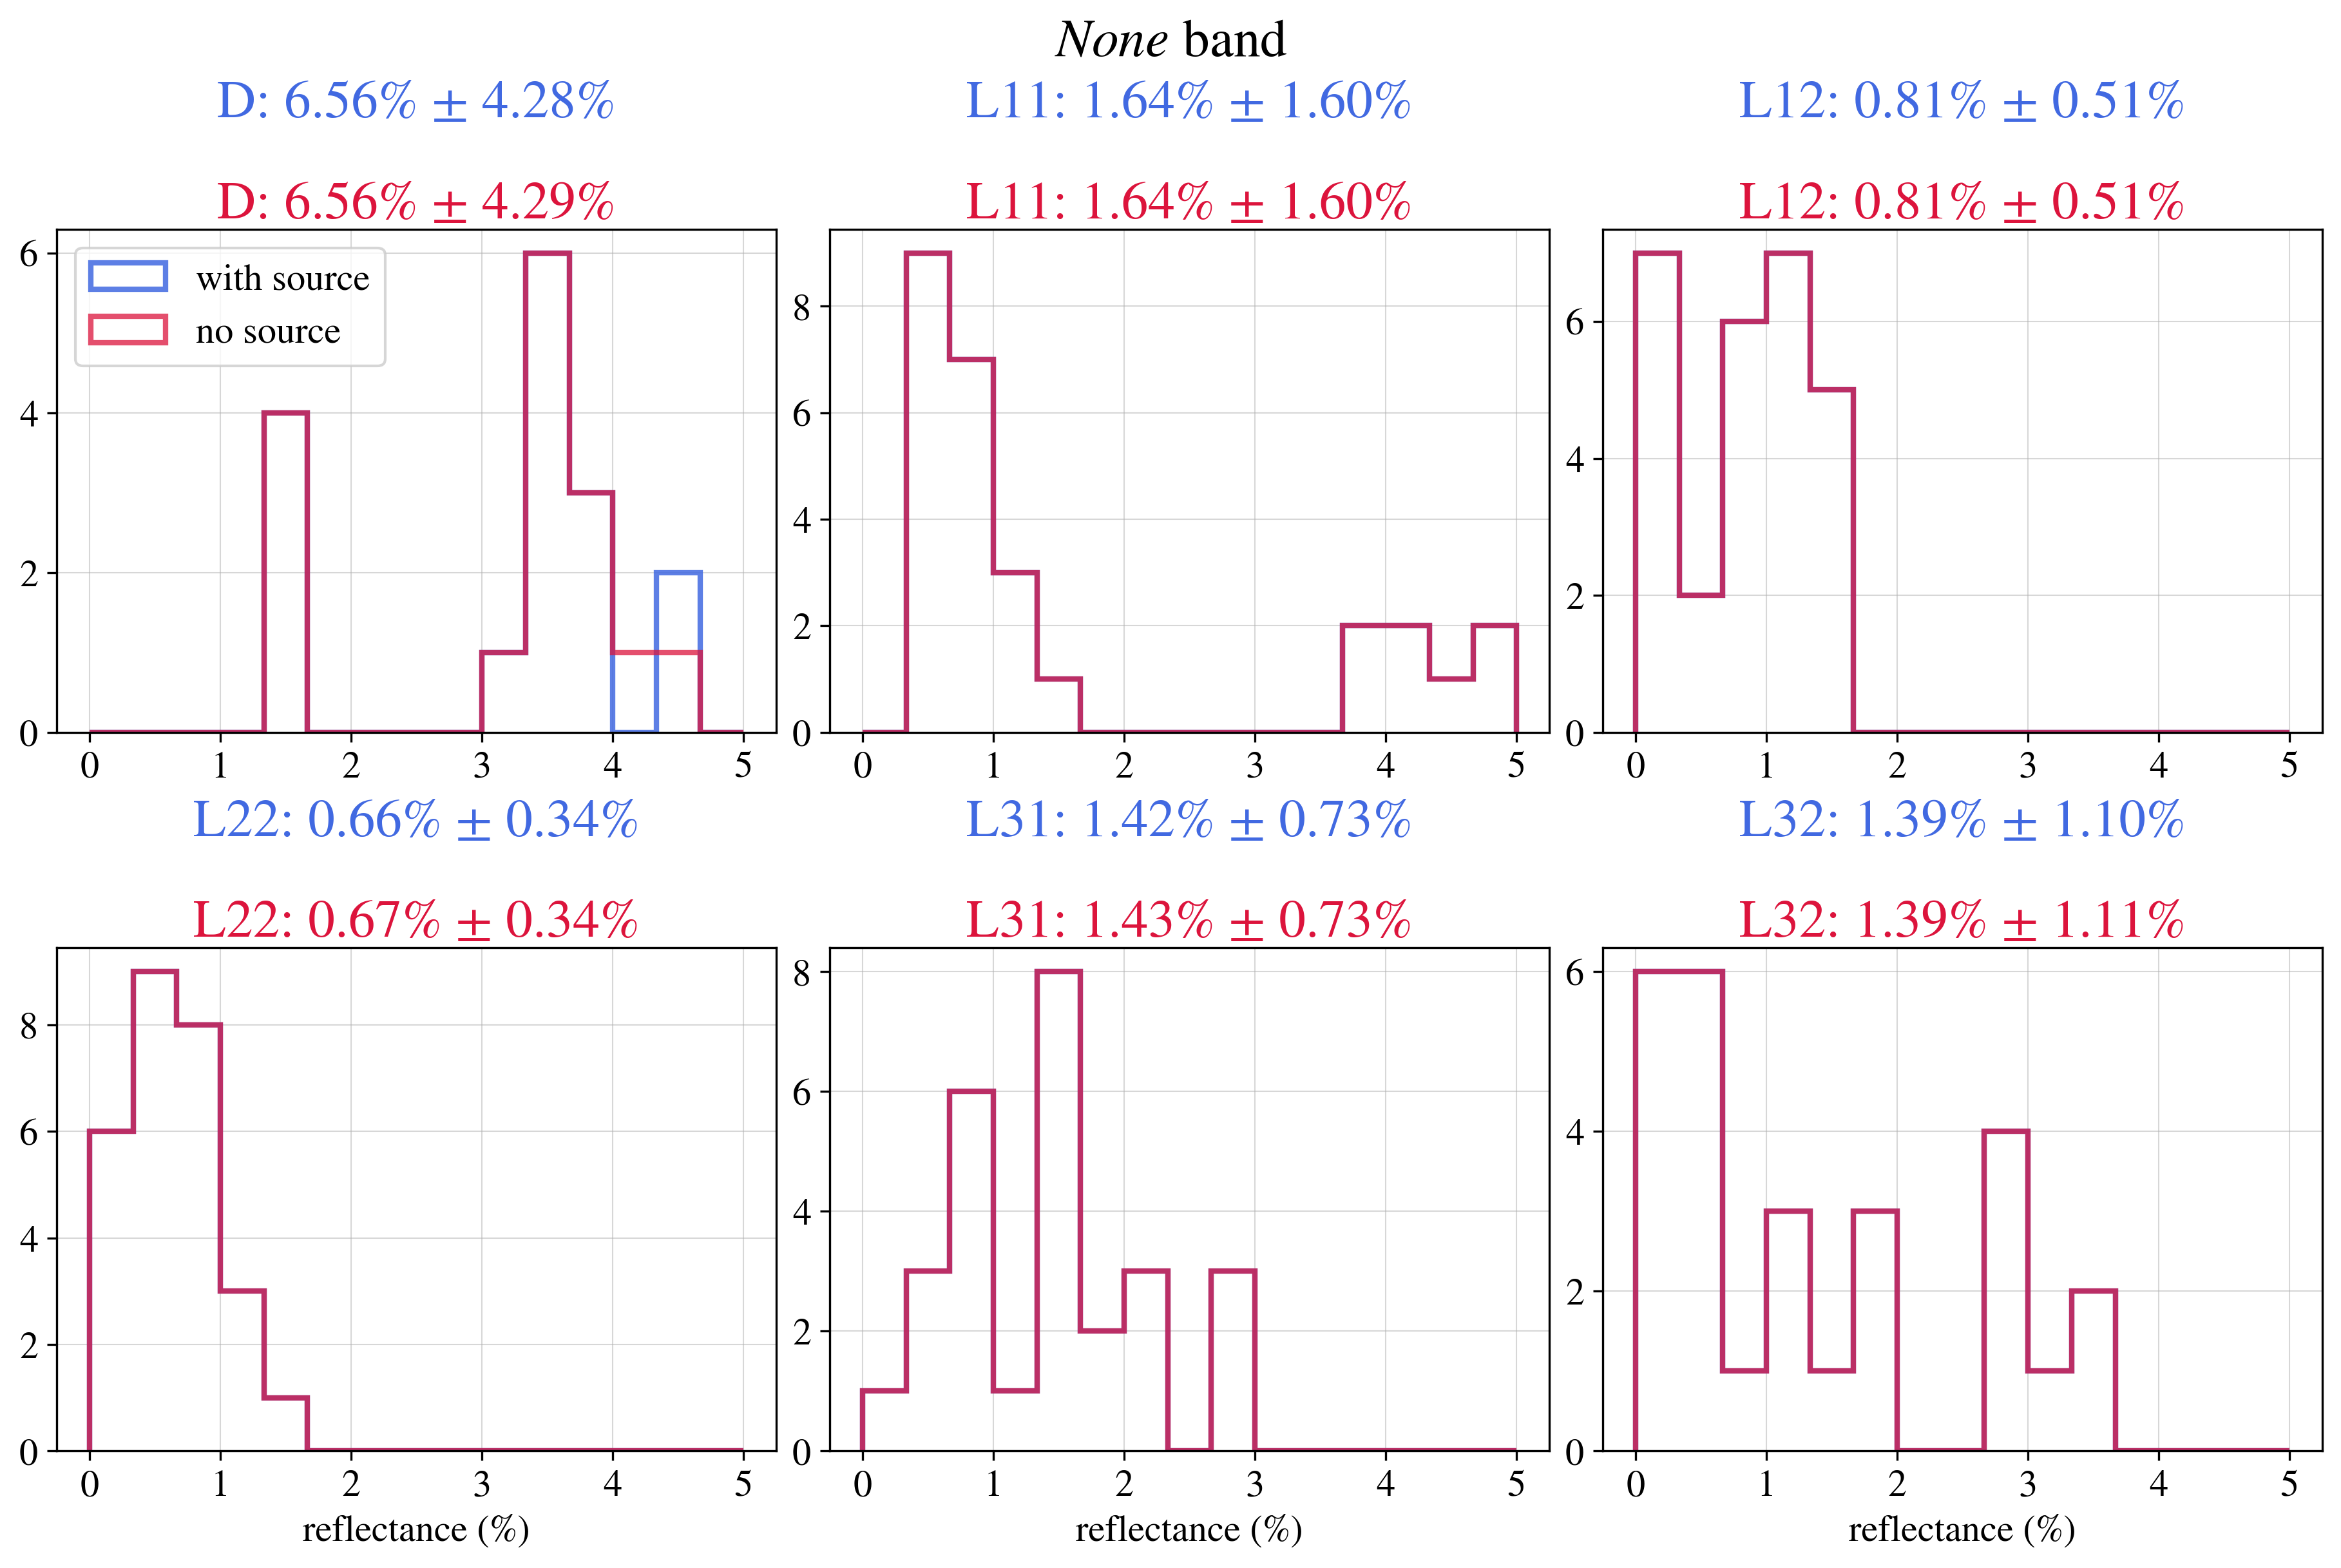
\includegraphics[width=\linewidth]{figures/None_reflectances.png}
    \caption{No filter}
    \label{subfig:refl_a}
  \end{subfigure}
  \medskip
  \begin{subfigure}[t]{0.8\textwidth}
    \centering
    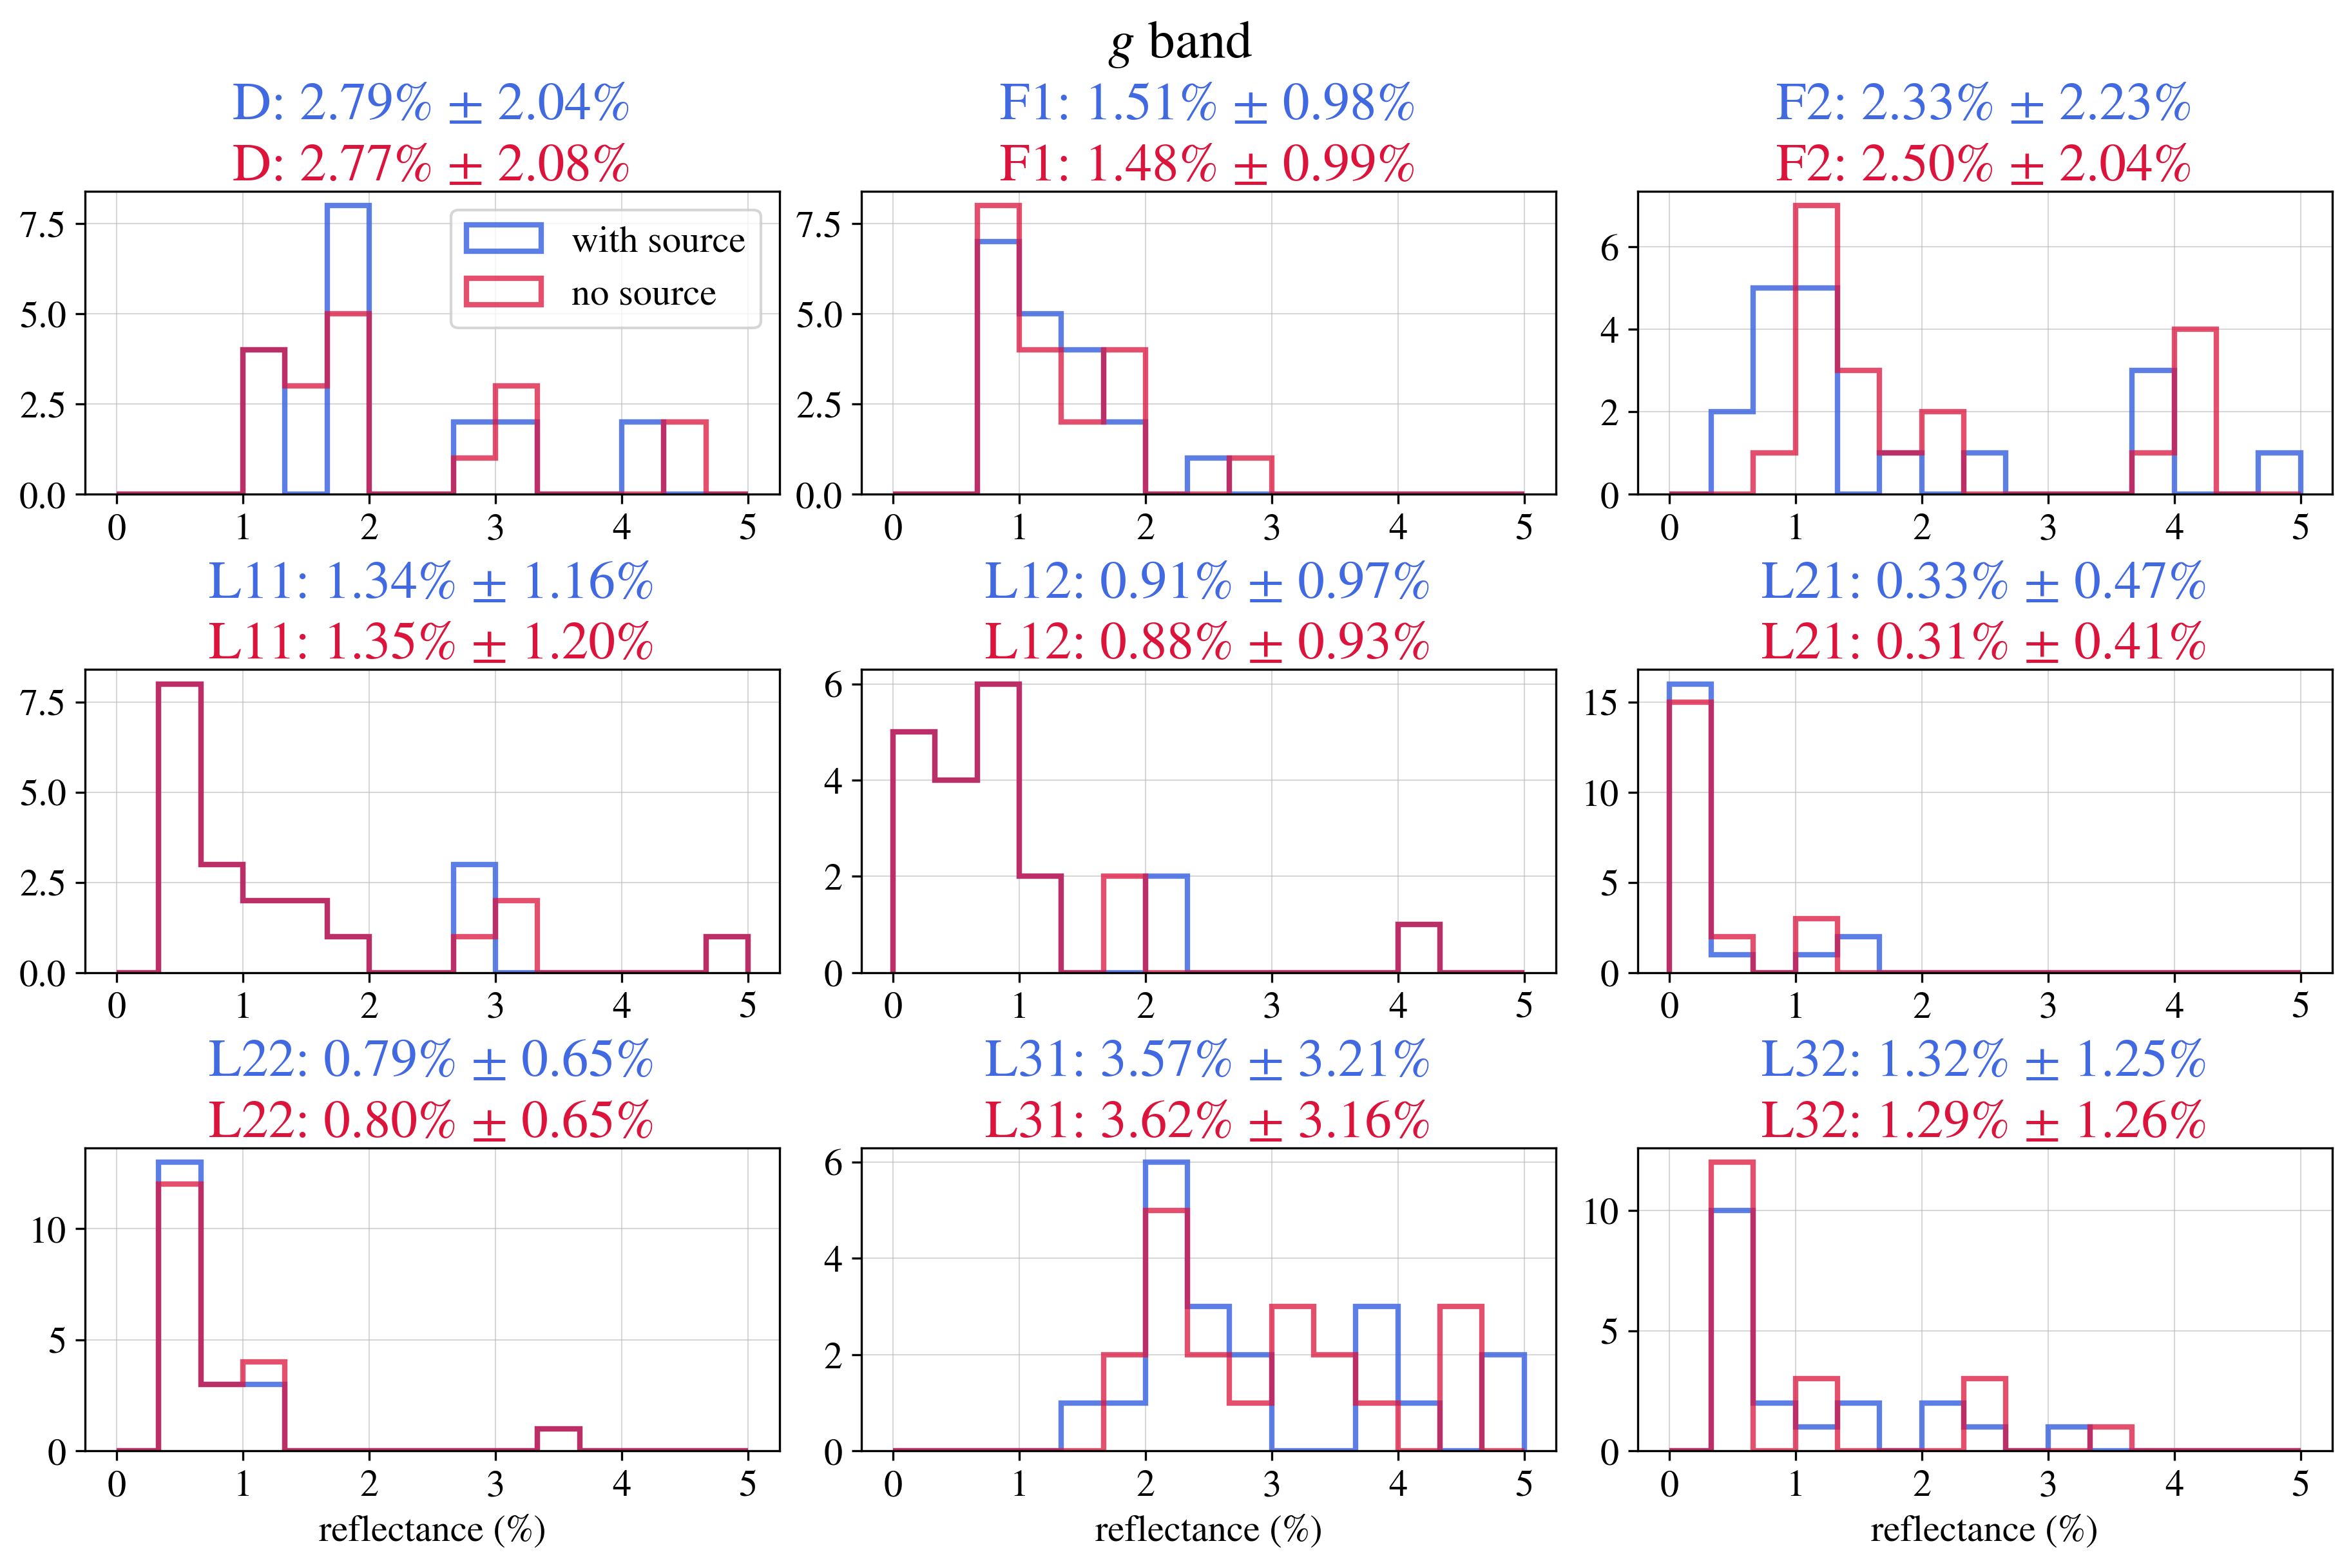
\includegraphics[width=\linewidth]{figures/g_reflectances.png}
    \caption{$g$ band}
    \label{subfig:refl_b}
  \end{subfigure}

  \caption{Distributions of reflectance measurements per visit separated by optic in the no-filter and {\it g} bands.
  The blue measurements are made including a fit to the source and the red measurements are made while masking the source.}
  \label{fig:reflectances_a}
\end{figure}

\begin{figure}[h!]
  \centering

  \begin{subfigure}[t]{0.8\textwidth}
    \centering
    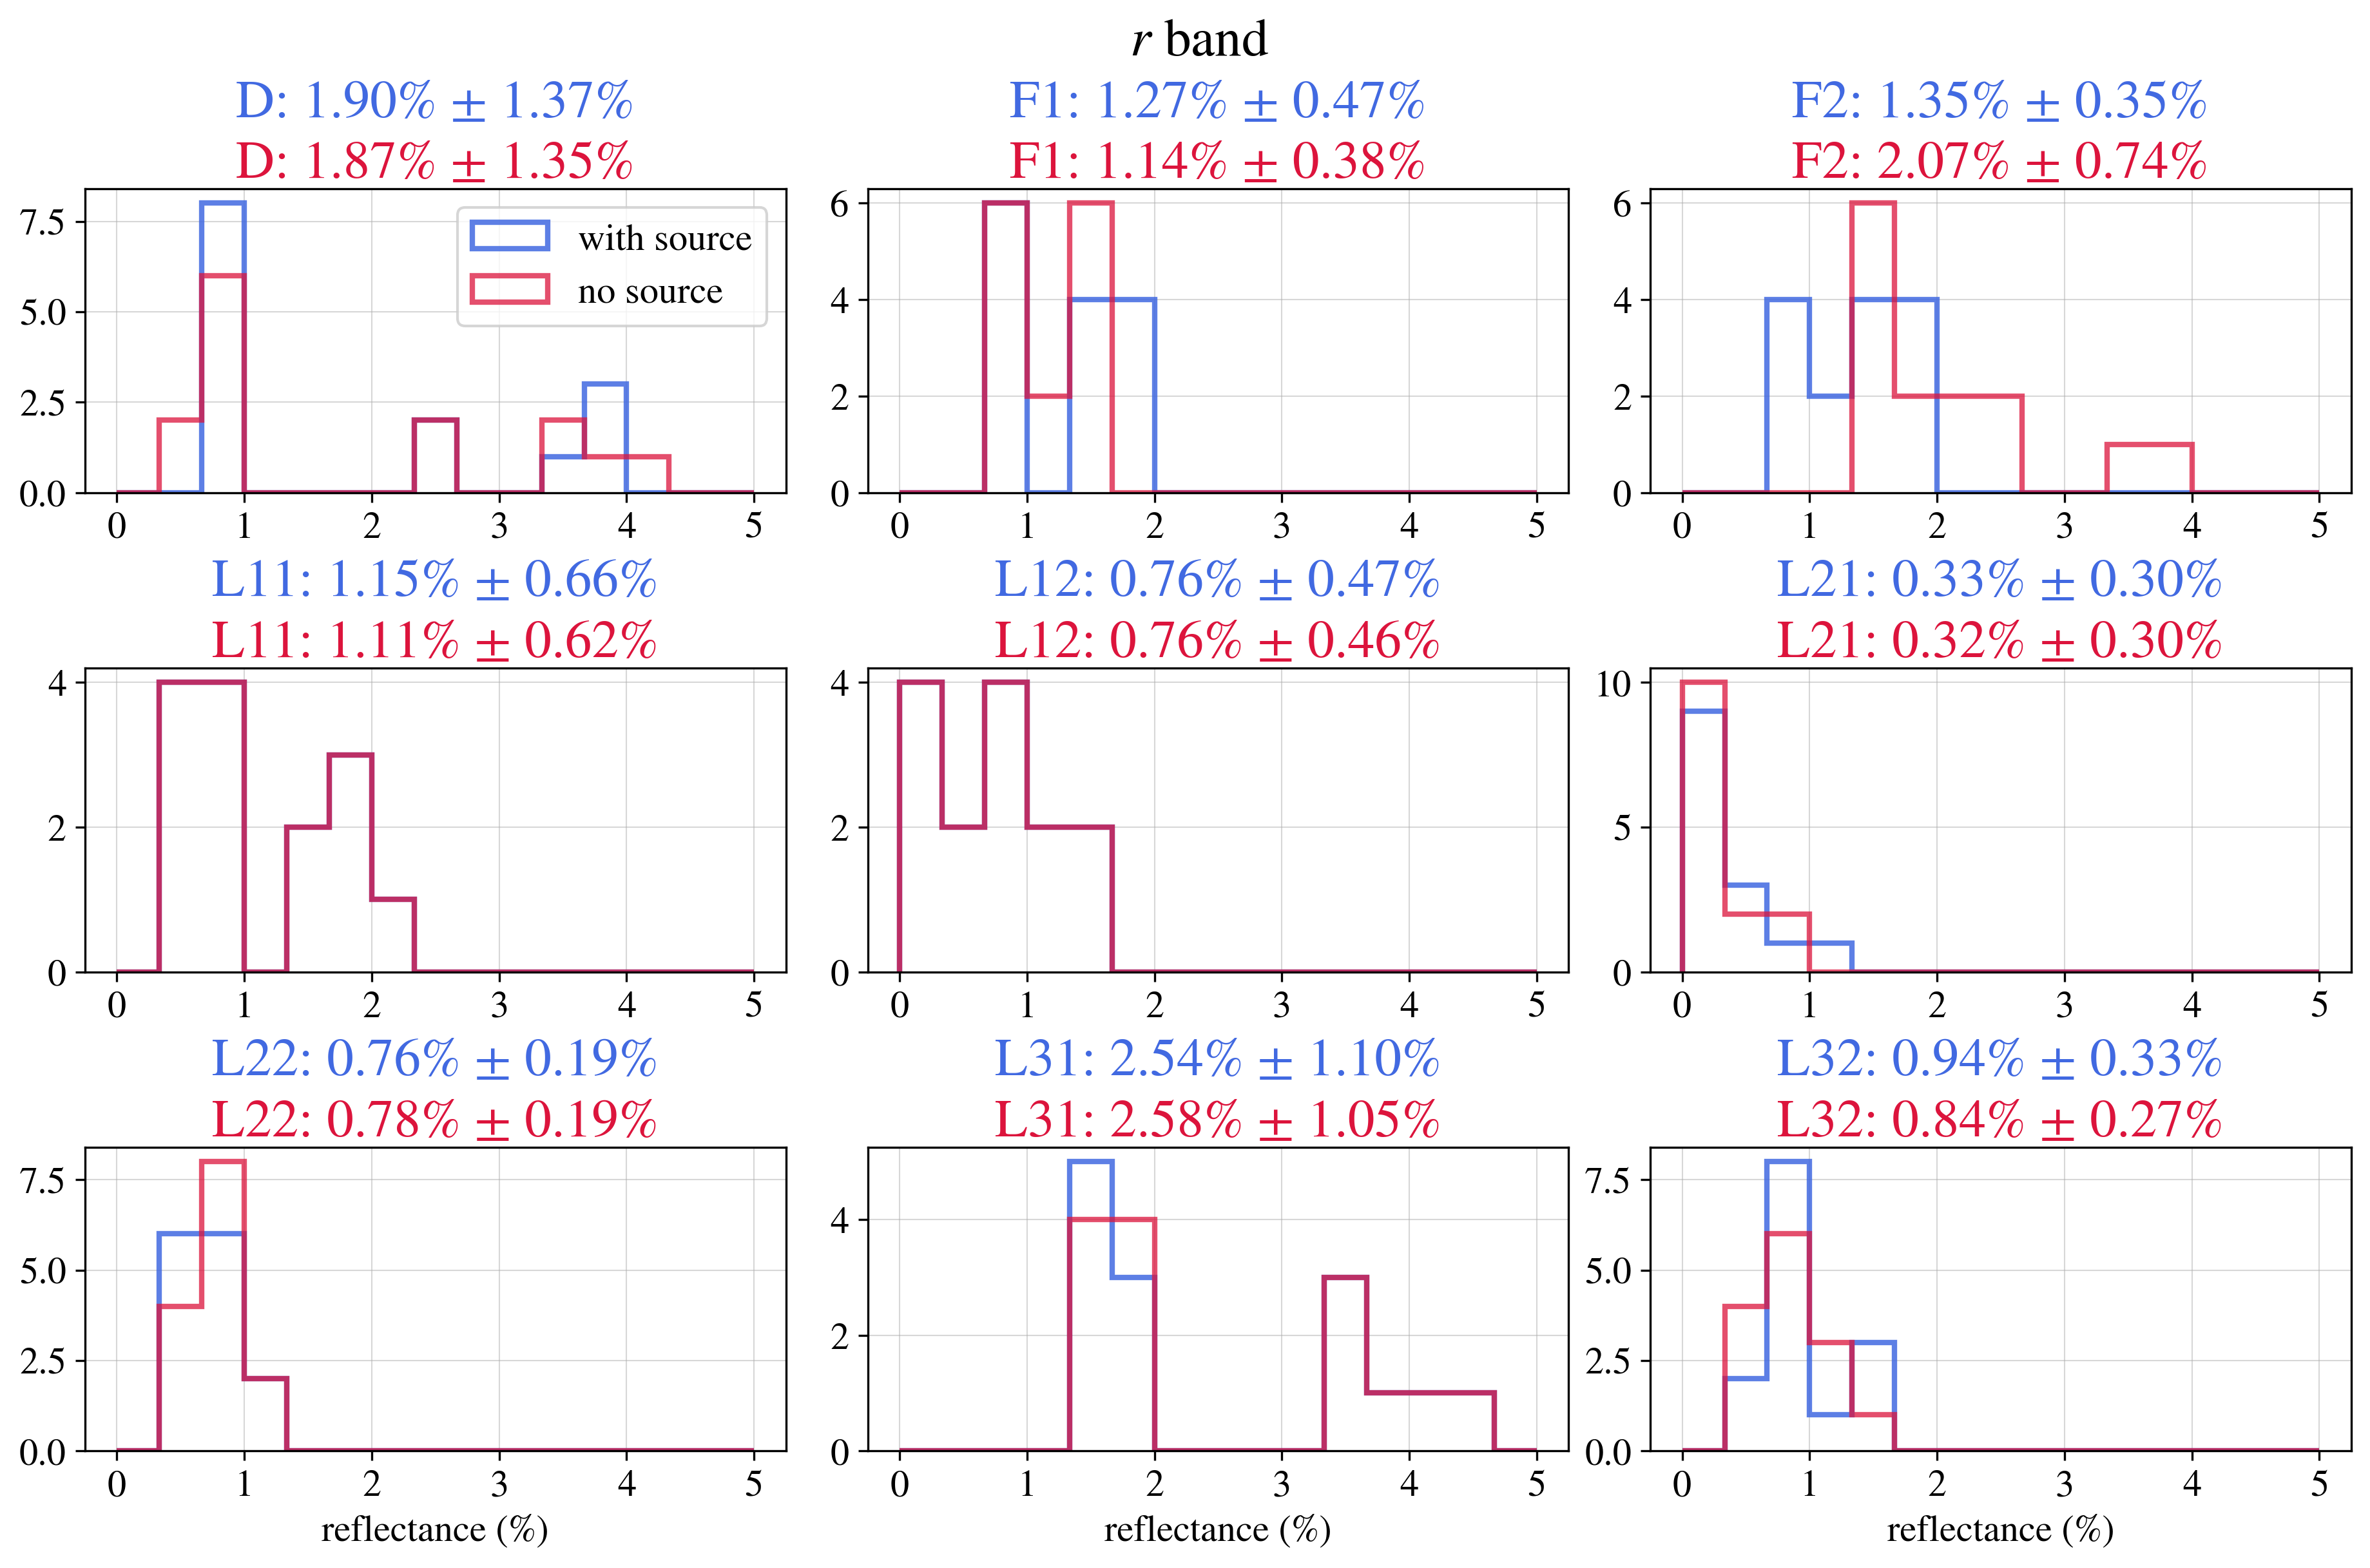
\includegraphics[width=\linewidth]{figures/r_reflectances.png}
    \caption{$r$ band}
    \label{subfig:refl_c}
  \end{subfigure}
 \medskip
  \begin{subfigure}[t]{0.8\textwidth}
    \centering
    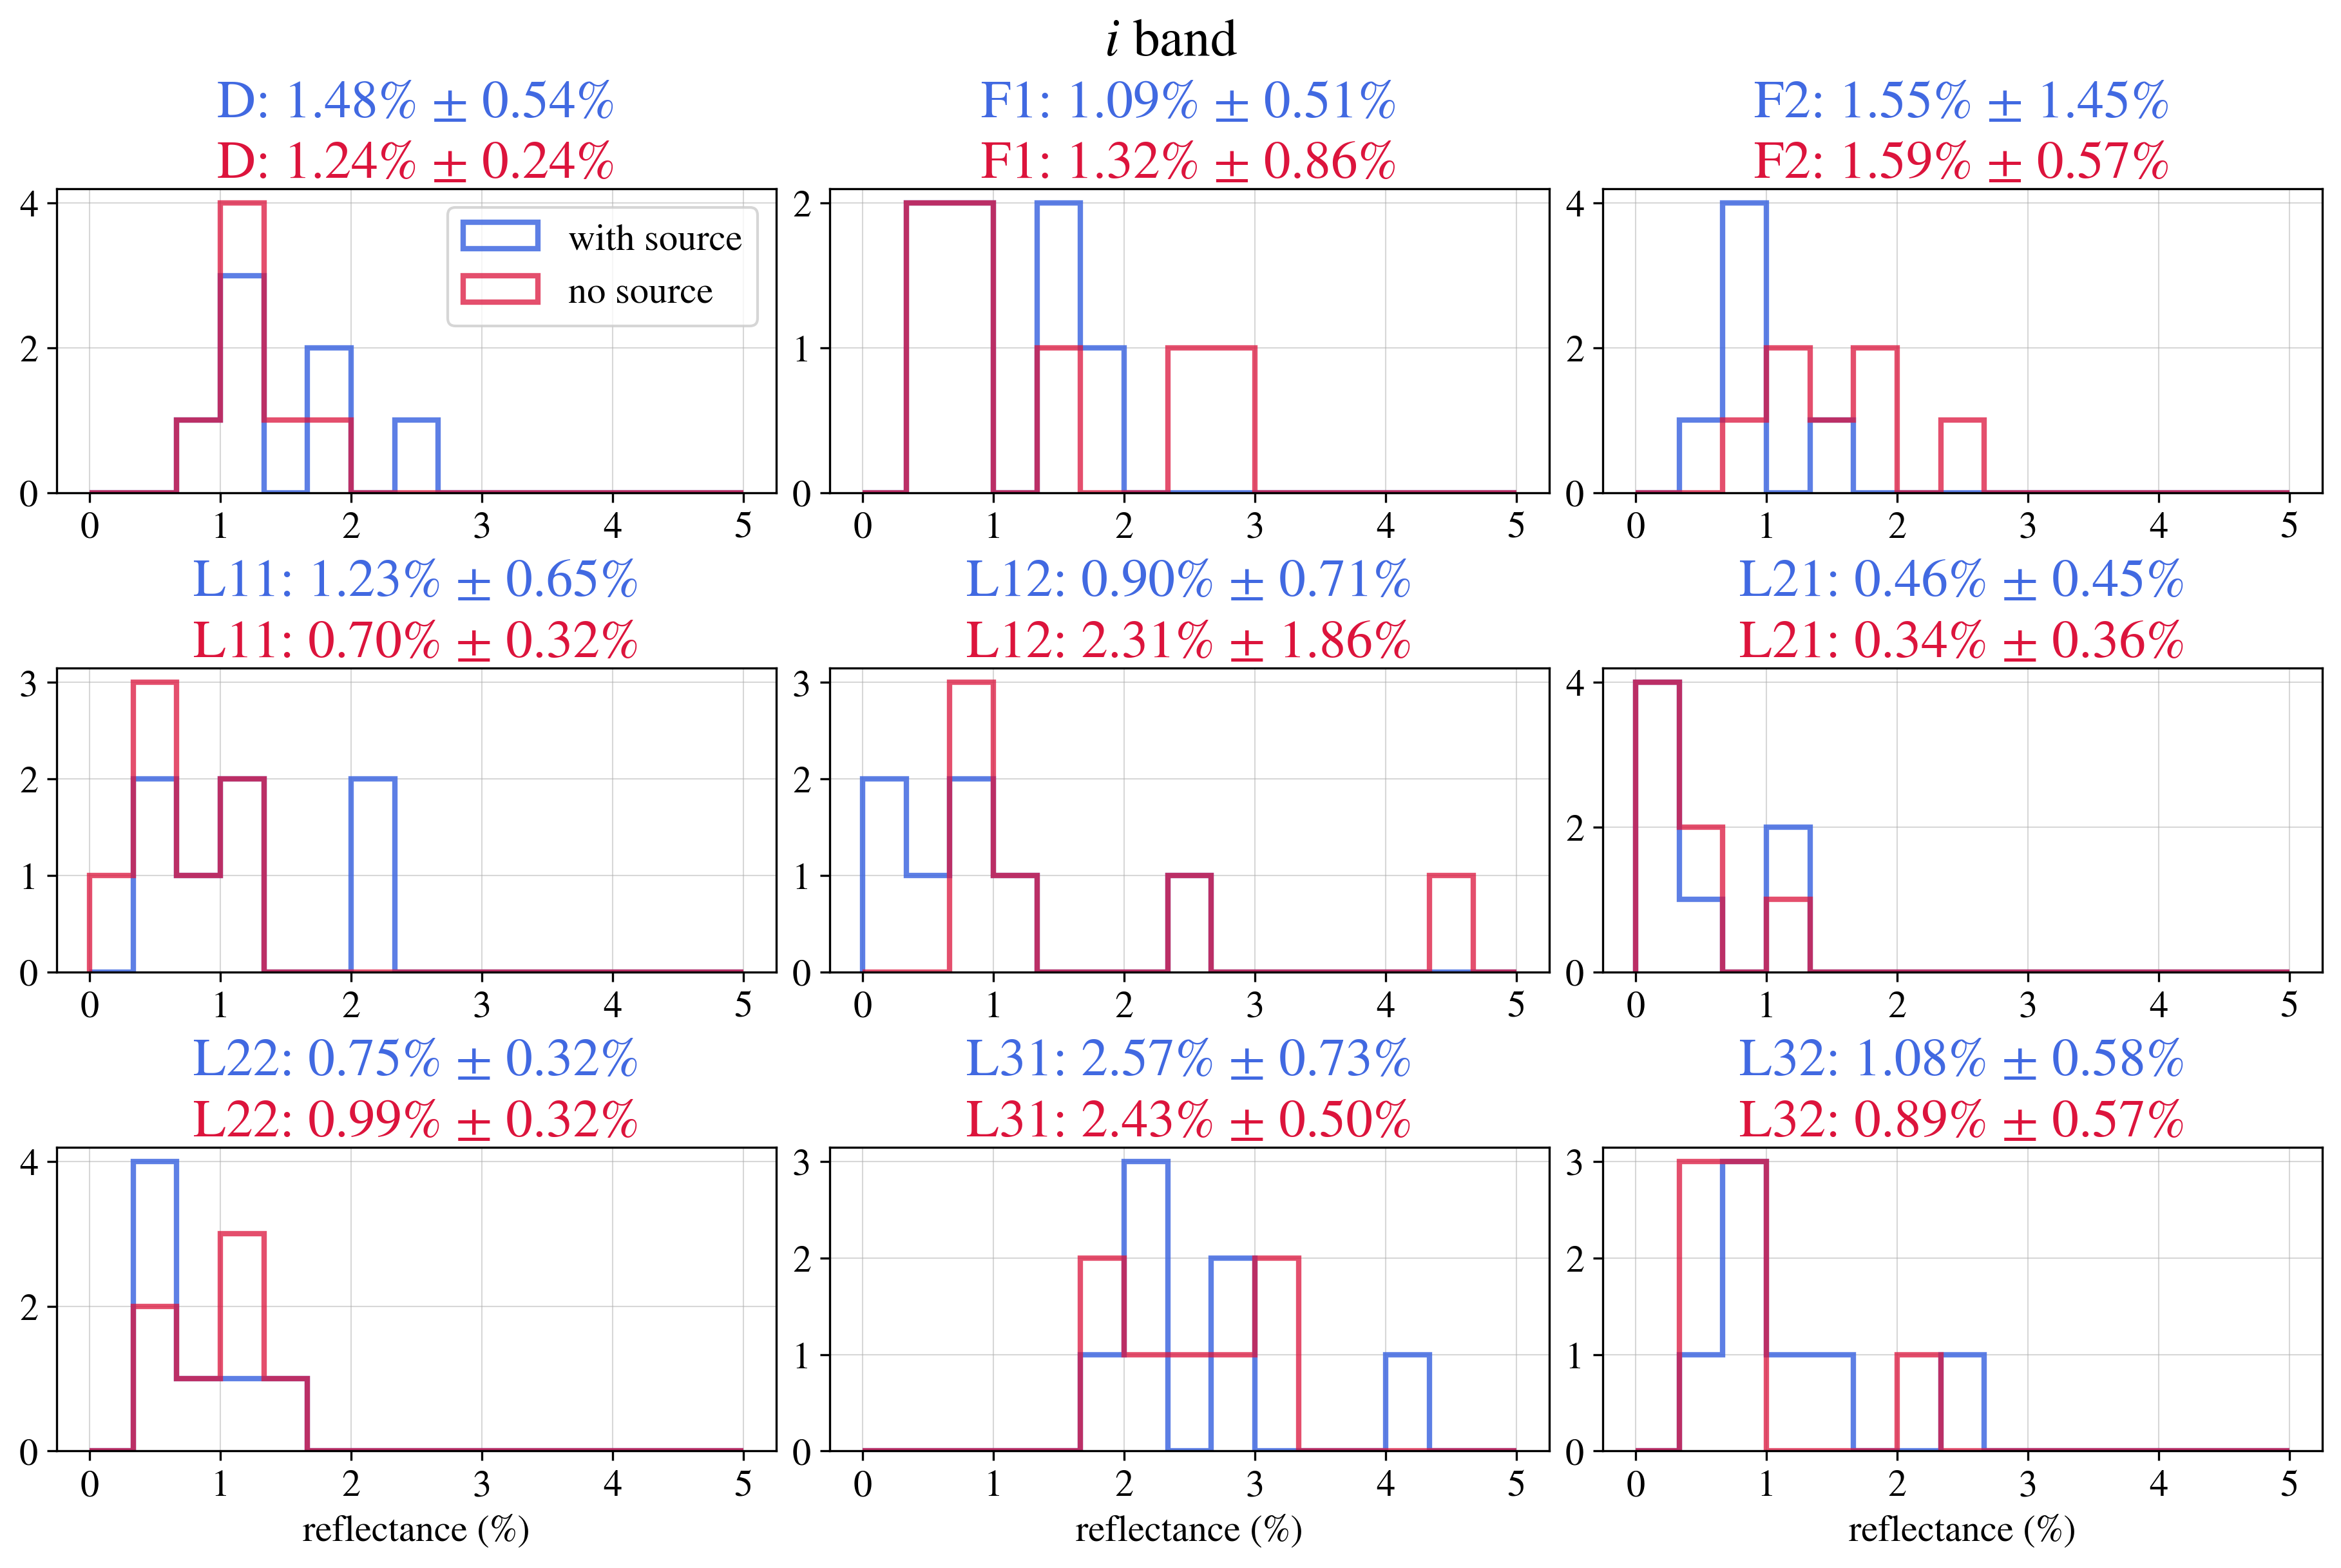
\includegraphics[width=\linewidth]{figures/i_reflectances.png}
    \caption{$i$ band}
    \label{subfig:refl_d}
  \end{subfigure}

  \caption{Distributions of reflectance measurements per visit separated by optic in the {\it r} and {\it i} bands.
  The blue measurements are made including a fit to the source and the red measurements are made while masking the source.}
  \label{fig:reflectances_b}
\end{figure}


